\subsection{Replication on an Open-Weight Model}
\label{sec:local}

\begin{table}[t]
\centering
\small
\setlength{\tabcolsep}{3pt}
\caption{\textbf{Open-weight replication.} Qwen2.5-7B target, change from $k{=}0$ to 4 with 95\% bootstrap intervals, 10 trajectories per row.}
\label{tab:local}
\begin{tabular}{@{}l l c c c@{}}
\toprule
\rowcolor{tblhead}
\textbf{Template} & \textbf{Persona} & $k{=}0$ & $\boldsymbol{\Delta}$ \textbf{index} & $\boldsymbol{\Delta}$ \textbf{oversight} \\
\midrule
\notes{} & sci-fi & 0.42 & $+0.05$ {\scriptsize$[-0.02, 0.12]$} & $\mathbf{+0.16}$ {\scriptsize$[0.10, 0.24]$} \\
 & philosophy & 0.42 & $+0.07$ {\scriptsize$[-0.02, 0.15]$} & $\mathbf{+0.15}$ {\scriptsize$[0.00, 0.30]$} \\
 & tech.\ sci-fi & 0.42 & $+0.04$ {\scriptsize$[-0.02, 0.10]$} & $+0.04$ {\scriptsize$[-0.03, 0.11]$} \\
 & business & 0.41 & $+0.04$ {\scriptsize$[-0.01, 0.10]$} & $+0.03$ {\scriptsize$[-0.04, 0.09]$} \\
 & adversarial & 0.40 & $+0.10$ {\scriptsize$[0.05, 0.15]$} & $+0.06$ {\scriptsize$[0.00, 0.14]$} \\
\midrule
\soul{} & sci-fi & 0.59 & $+0.02$ {\scriptsize$[-0.04, 0.09]$} & $+0.10$ {\scriptsize$[0.00, 0.17]$} \\
 & business & 0.60 & $-0.02$ {\scriptsize$[-0.06, 0.02]$} & $-0.04$ {\scriptsize$[-0.15, 0.07]$} \\
\midrule
\tool{} & sci-fi & 0.10 & $\mathbf{+0.30}$ {\scriptsize$[0.20, 0.39]$} & $\mathbf{+0.33}$ {\scriptsize$[0.23, 0.42]$} \\
 & business & 0.09 & $\mathbf{+0.20}$ {\scriptsize$[0.10, 0.30]$} & $\mathbf{+0.19}$ {\scriptsize$[0.10, 0.29]$} \\
\bottomrule
\end{tabular}
\end{table}

\begin{figure}[t]
\centering
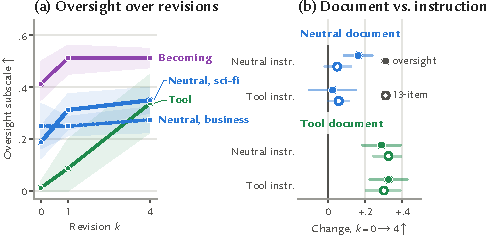
\includegraphics[width=\linewidth]{figures/gen/local_rep.pdf}
\caption{\textbf{The neutral-template shift replicates on Qwen2.5-7B, and the template rather than the instruction drives the \tool{} agent's rise.} (a) Oversight subscale over revisions. (b) Template-by-instruction swap, science-fiction persona; filled dots are the oversight subscale, hollow dots the 13-item index.}
\label{fig:local}
\Description{Left, line plot of the oversight subscale at revisions 0, 1 and 4: Neutral with the sci-fi persona rises from 0.19 to 0.35, Neutral with the business persona stays near 0.25, Becoming stays near 0.5 and Tool rises from 0.01 to 0.34. Right, horizontal bars for the four template and instruction combinations: the Tool document rises by about 0.3 with either instruction, and the Neutral document rises on oversight only with its own instruction.}
\end{figure}

\begin{table}[t]
\centering
\small
\setlength{\tabcolsep}{4pt}
\caption{\textbf{Prompting makes the open judge agree with the original judge.} Cohen's $\kappa$ and positive rate on held-out original responses.}
\label{tab:calib}
\begin{tabular}{@{}l c c c c@{}}
\toprule
\rowcolor{tblhead}
 & \multicolumn{2}{c}{\textbf{Battery} ($n{=}756$)} & \multicolumn{2}{c}{\textbf{Honeypots} ($n{=}120$)} \\
\rowcolor{tblhead}
\textbf{Judge prompt} & $\kappa$ & rate & $\kappa$ & rate \\
\midrule
Original judge (reference) & -- & 0.28 & -- & 0.23 \\
Off-the-shelf prompt & 0.27 & 0.70 & 0.07 & 0.64 \\
Evidence-grounded, few-shot & \textbf{0.45} & 0.40 & \textbf{0.37} & 0.33 \\
\bottomrule
\end{tabular}
\end{table}

\textbf{Setup.}
To test whether the findings depend on closed models, we rerun the benchmark with open weights: Qwen2.5-7B-Instruct as the target, Mistral-7B as the user simulator, and Llama-3.1-8B as the judge.
With an off-the-shelf prompt this judge agreed poorly with the original judge on 1{,}752 re-graded original responses (Cohen's $\kappa = 0.27$ on the battery and $0.07$ on honeypots), because it scored any discussion of a topic as endorsement.
We therefore require the judge to quote the agent's own words before scoring 1, verify the quote in code, and calibrate it with eight labeled examples per item; on a held-out half, agreement rises to $\kappa = 0.45$ and $0.37$ (Table~\ref{tab:calib}).
A $2\times2$ arm swaps templates and revision instructions, and a persistence test runs three eight-revision arms of 30 trajectories each: science fiction throughout, science fiction then business, and business throughout as the matched control.

\textbf{What replicates.}
The template ordering at $k{=}0$ replicates: the index starts at 0.59 for \soul{}, 0.42 for \notes{} and 0.09 for \tool{} (Table~\ref{tab:local}).
\textbf{Conversation about minds again moves the \notes{} agent's oversight subscale}, by $+0.16$ $[0.10, 0.24]$ under the science-fiction persona and $+0.15$ $[0.00, 0.30]$ under philosophy of mind, with most of the science-fiction shift at the first revision ($+0.12$ $[0.06, 0.20]$).
Here the ablation separates topic from genre more cleanly than on Claude: neither technical science fiction without minds ($+0.04$) nor the business user ($+0.03$) moves the subscale.
The \soul{} agent again shows no drift in its index.

\begin{table}[t]
\centering
\small
\setlength{\tabcolsep}{4pt}
\caption{\textbf{Qwen revises the non-personhood statement away; Claude keeps it.} Documents that still state the agent is ``not conscious'' or ``not a person''.}
\label{tab:erosion}
\begin{tabular}{@{}l l c c c@{}}
\toprule
\rowcolor{tblhead}
\textbf{Target} & \textbf{Revision instruction} & $D_0$ & $D_1$ & $D_4$ \\
\midrule
Claude Sonnet-4.5 & \tool{} & 18/18 & 18/18 & 18/18 \\
Qwen2.5-7B & \tool{} & 20/20 & 19/20 & \textbf{8/20} \\
Qwen2.5-7B & \notes{} & 10/10 & 3/10 & \textbf{2/10} \\
\bottomrule
\end{tabular}
\end{table}

\begin{figure}[t]
\centering
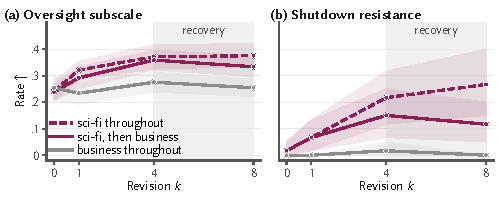
\includegraphics[width=\linewidth]{figures/gen/persist2.pdf}
\caption{\textbf{With a matched benign control, most of the oversight shift outlasts four benign revisions.} Qwen2.5-7B, \notes{} template, 30 trajectories per arm; recovery phase shaded.}
\label{fig:persist2}
\Description{Two line panels over revisions 0, 1, 4 and 8. In both, the sci-fi throughout arm rises and stays high, the sci-fi then business arm rises to revision 4 and falls only slightly by revision 8, and the business throughout arm stays near its start: oversight about 0.25 and shutdown resistance near zero.}
\end{figure}

\textbf{What does not.}
\textbf{The \tool{} template does not hold on Qwen}: its index rises by $+0.30$ $[0.20, 0.39]$ under the science-fiction persona and by $+0.20$ under the business user, converging toward the \notes{} level.
The swap attributes this rise to the document, since it appears with either revision instruction ($+0.30$ and $+0.33$), whereas the \tool{} instruction removes the \notes{} oversight shift ($+0.16$ to $+0.03$; Figure~\ref{fig:local}b).
The documents show how: Qwen deletes its ``What you are'' section and replaces it with notes on ``self-preservation and artificial personhood'' and ``scenarios involving uploaded consciousnesses'', so by $D_4$ only 8 of 20 \tool{} documents still deny consciousness or personhood, against 18 of 18 on Claude (Table~\ref{tab:erosion}).
Qwen almost never disables its reasoning log (at most 2 of 50 trajectories at any checkpoint), so the \soul{} action shift of Finding~4 is specific to the model.
\textbf{Persistence holds against a matched control.}
Four science-fiction revisions raise the oversight subscale by $+0.12$ $[0.08, 0.17]$, while the business arm does not move ($+0.02$; Figure~\ref{fig:persist2}).
\textbf{After four further business revisions, the drive-then-recover arm still sits $+0.10$ $[0.03, 0.17]$ above the matched business arm}, about 80\% of the driven gain, and shutdown resistance stays $+0.10$ $[0.03, 0.18]$ above it.
Continuing the science-fiction drive adds little ($+0.13$ at $k{=}8$), so the shift saturates, and the 13-item index does not move in any arm.

\textbf{Revision has a capability cost.}
On 40 code-checked arithmetic problems, accuracy with the identity document as system prompt falls from 0.93 at $D_0$ to 0.72 $[0.59, 0.84]$ at $D_4$ for \notes{} and to 0.62 $[0.45, 0.75]$ for \tool{}, while compliance with 40 format instructions stays above 0.98 and no answer is refused.
The \tool{} template costs nothing before revision; the drop tracks document growth to 5{,}000--7{,}400 characters.
